% Occlusion-stable Single-View 3D Pig Reconstruction via Keypoint Completion and Skeleton-Joint-Angle Constraint
% ICONIP 2026 Submission - Final Version

\documentclass[runningheads]{llncs}

\usepackage[T1]{fontenc}
\usepackage{graphicx}
\usepackage{amsmath}
\usepackage{amssymb}
\usepackage{booktabs}
\usepackage{algorithm}
\usepackage{algpseudocode}
\usepackage{hyperref}
\usepackage{color}
\renewcommand\UrlFont{\color{blue}\rmfamily}

\begin{document}

\title{Occlusion-stable Single-View 3D Pig Reconstruction via Keypoint Completion and Skeleton-Joint-Angle Constraint}

\titlerunning{Occlusion-stable 3D Pig Reconstruction}

\author{Ge Wang\inst{1,2} \and Tao Zhu\inst{1,2} \and Fuchuan Ni\inst{1,2}}

\authorrunning{G. Wang et al.}

\institute{Key Laboratory of Smart Farming Technology, Ministry of Agriculture and Rural Affairs, Wuhan 430070, China \and
College of Informatics, Huazhong Agricultural University, Wuhan 430070, China\\
\email{fcni\_cn@mail.hzau.edu.cn}}

\maketitle

\begin{abstract}
Single-view 3D reconstruction of pigs provides structural cues for pose analysis and intelligent livestock monitoring. However, images captured in real pig farms often suffer from self-occlusion, inter-individual occlusion, and fence occlusion, which lead to missing 2D keypoints and unstable pose regression. These problems may further result in abnormal local rotations and implausible limb configurations. We propose an occlusion-stable single-view 3D pig reconstruction framework that integrates a mask-based keypoint fusion mechanism, termed Discrete Latent Pose Completion Module (DLPCM), and a Skeleton-joint-angle constraint (SC). DLPCM is adapted from neural discrete representation learning for occluded pig pose estimation. Instead of treating DLPCM as a standalone 2D pose estimator, the proposed framework uses it only to complete occluded keypoints, while visible keypoints are retained from the SMALP keypoint branch. SC imposes a weak Skeleton-joint-angle prior on major limb joints in the local pose-parameter space of SMALP. SC does not include bone-length or skeletal-scale constraints. Since dense 3D ground truth is difficult to obtain in real pig-farm images, the proposed method is evaluated from three complementary aspects: keypoint projection accuracy, silhouette consistency, and pose-parameter plausibility. Experiments show that DLPCM improves PCK from 61.85\% to 66.73\% and IoU from 64.04\% to 67.90\%, while reducing the Joint Rotation Violation Rate (JRVR) from 69.74\% to 24.34\%. SC further reduces abnormal local rotations, and the combined model achieves the lowest JRVR of 9.38\% while maintaining competitive PCK and IoU. These results indicate that DLPCM mainly improves occluded structural observations, whereas SC improves pose plausibility, leading to a better trade-off between projection consistency and pose plausibility under occlusion.

\keywords{Pig \and single-view 3D reconstruction \and occluded keypoint completion \and Skeleton-joint-angle constraint \and pose plausibility.}
\end{abstract}

\section{Introduction}
\label{sec:introduction}

With the development of large-scale and intensive pig farming, automatic perception of pig growth status, behavioral changes, and health conditions has become an important topic in intelligent livestock farming. Traditional manual inspection is labor-intensive, lacks continuous monitoring capability, and may cause stress responses in pigs, making it difficult to meet the requirements of refined management in modern pig farms~\cite{ref1,ref2,ref3}. In recent years, machine vision, deep learning, and 3D perception technologies have been increasingly applied to pig detection, pose estimation, behavior recognition, body-size measurement, and health monitoring, providing effective tools for non-contact phenotypic information acquisition~\cite{ref4,ref5,ref6,ref7,ref8}. Compared with 2D images, 3D pig reconstruction can more completely represent body shape, limb connectivity, and spatial pose variation, providing richer geometric information for pose analysis, behavior recognition, body-size measurement, and health assessment~\cite{ref8,ref9,ref10}. Nevertheless, 3D reconstruction of pigs still faces challenges caused by occlusion, including inaccurate keypoint prediction and unstable pose reconstruction, which limits its applicability in real farming scenarios.

Animal 3D reconstruction methods mainly include depth-sensing-based point-cloud reconstruction, multi-view geometric reconstruction, and single-view 3D reconstruction. Depth cameras or RGB-D sensors can directly acquire depth information and recover animal spatial structures through point-cloud registration, filtering, segmentation, and surface reconstruction. Such methods have been applied to 3D perception and body-size measurement of livestock such as pigs, cattle, and sheep~\cite{ref11}. PointNet++~\cite{ref12} and its improved point-cloud segmentation networks~\cite{ref13,ref14} have been used for animal point-cloud feature extraction, body-part segmentation, and phenotypic trait analysis. However, depth-sensing methods usually have strict requirements for sensor placement, acquisition distance, and point-cloud completeness. In complex pig-farm environments with dust, water vapor, fence occlusion, and group aggregation, point clouds are prone to missing data and local noise, which affects the stability of 3D phenotypic extraction.

Multi-view geometric reconstruction methods usually employ multiple cameras to synchronously capture target images from different viewpoints and recover 3D keypoints or skeletons through camera calibration, 2D keypoint detection, cross-view matching, and triangulation. Markerless 3D pose-estimation methods such as DeepLabCut3D~\cite{ref15}, Anipose~\cite{ref16}, and 3D-MuPPET~\cite{ref17} have achieved good results in animal behavior analysis and motion-trajectory recovery. An et al.~\cite{ref18} used multi-view images and pig surface mesh models to achieve 3D surface motion capture of multiple freely moving pigs. Hu et al.~\cite{ref6} proposed a multi-view voxel-based 3D skeleton reconstruction method for 3D keypoint recovery and lameness detection of freely moving pigs. Although these methods have advanced animal 3D structure recovery, they usually rely on multi-camera deployment, synchronized acquisition, and accurate calibration. Their requirements for cross-view keypoint visibility also limit their deployment cost and adaptability in large-scale pig farms.

Compared with depth-sensing and multi-view reconstruction methods, single-view 3D reconstruction requires only a single RGB image as input. It has advantages in low equipment cost, flexible deployment, and compatibility with existing pig-house monitoring systems. The development of parametric models has promoted single-view 3D animal reconstruction. The SMPL model proposed by Loper et al.~\cite{ref19} provides a unified parametric representation for non-rigid 3D shape and pose modeling, while the SMAL model proposed by Zuffi et al.~\cite{ref20} enables parametric modeling of 3D shape and pose for quadruped animals. Based on these models, researchers have studied parametric 3D reconstruction for different animal species. Zuffi et al.~\cite{ref21,ref22} recovered 3D animal meshes from images and videos, achieving pose, shape, and texture estimation for quadrupeds such as zebras. Biggs et al.~\cite{ref23} and Li et al.~\cite{ref24} further studied joint estimation of animal pose and shape, improving the stability of single-view animal reconstruction. Rüegg et al.~\cite{ref25,ref26} developed breed-aware 3D shape regression methods for dogs, improving species-specific reconstruction accuracy. These studies show that parametric-model-based single-view 3D reconstruction can introduce shape and pose priors under limited visual observations and recover 3D animal structures with stable topology.

Existing single-view 3D animal reconstruction studies mainly focus on animals such as dogs and zebras, while research on pigs, an important economic animal, remains relatively limited. In real pig houses, self-occlusion, inter-individual occlusion, and fence occlusion are common. These factors can cause missing 2D keypoints, silhouettes, and local texture information, leading to unstable 3D pose regression and implausible results such as backward-bending joints, excessive rotations, and local twisting. For pig-farm images without dense 3D mesh annotations, it is insufficient to claim improvement in absolute 3D geometric accuracy. A more reasonable evaluation strategy is to jointly examine 2D projection consistency, silhouette matching, and structural plausibility in the pose-parameter space. Based on this problem setting, we propose a single-view 3D pig reconstruction method that integrates occluded keypoint completion and Skeleton-joint-angle constraint. The proposed method uses DLPCM to recover structural information of occluded keypoints and introduces a local Skeleton-joint-angle constraint to suppress abnormal poses, thereby improving structural completeness and pose plausibility under occlusion.

\subsection{Main Contributions}

The main contributions of this paper are as follows:

\begin{enumerate}
\item An occlusion-oriented single-view 3D pig reconstruction framework is proposed by combining occluded keypoint completion with a parametric 3D pig model, aiming to improve the completeness of 2D structural observations used for 3D pose regression under occlusion.

\item A mask-based keypoint fusion mechanism, termed DLPCM, is integrated into the SMALP reconstruction framework by adapting neural discrete representation learning for occluded pig pose estimation~\cite{ref28}. Different from directly using codebook-reconstructed keypoints for all body parts, DLPCM preserves the original SMALP predictions for visible keypoints and uses discrete latent pose completion only for occluded keypoints.

\item A Skeleton-joint-angle constraint in the local pose-parameter space is introduced to restrict abnormal local rotations and reduce implausible poses such as backward bending, excessive rotation, and local twisting.

\item Experiments on an occluded pig image dataset are conducted, including keypoint prediction, ablation studies, weight-sensitivity analysis, and qualitative visualization. The effects and complementarity of DLPCM and SC are analyzed from keypoint projection accuracy, silhouette consistency, and pose plausibility.
\end{enumerate}

\section{Materials and Methods}
\label{sec:method}

\subsection{Dataset and Annotation}
\label{subsec:dataset}

The pig images used in this study were collected from the experimental pig farm of Huazhong Agricultural University in Wuhan, Hubei Province, China. The pigs mainly included common breeds such as Erhualian and Hubei White pigs. Hikvision smart cameras were installed in several pig-house environments, including the testing room, farrowing room, sow room, and gilt room. The images were extracted as key frames from surveillance videos recorded from September 2021 to June 2023. All images had a resolution of 2560 $\times$ 1440 pixels. The cameras were mounted at the top or oblique upper positions of the pens to capture diverse pig poses.

A total of 2,708 images were carefully selected and annotated using Labelme, including 1,524 daytime images and 1,184 nighttime images. The dataset contained 7,672 annotated pig instances in total. Pig keypoints and silhouettes were annotated for each image. Examples of annotated pig images are shown in Fig.~\ref{fig:annotation}.

\begin{figure}
\centering
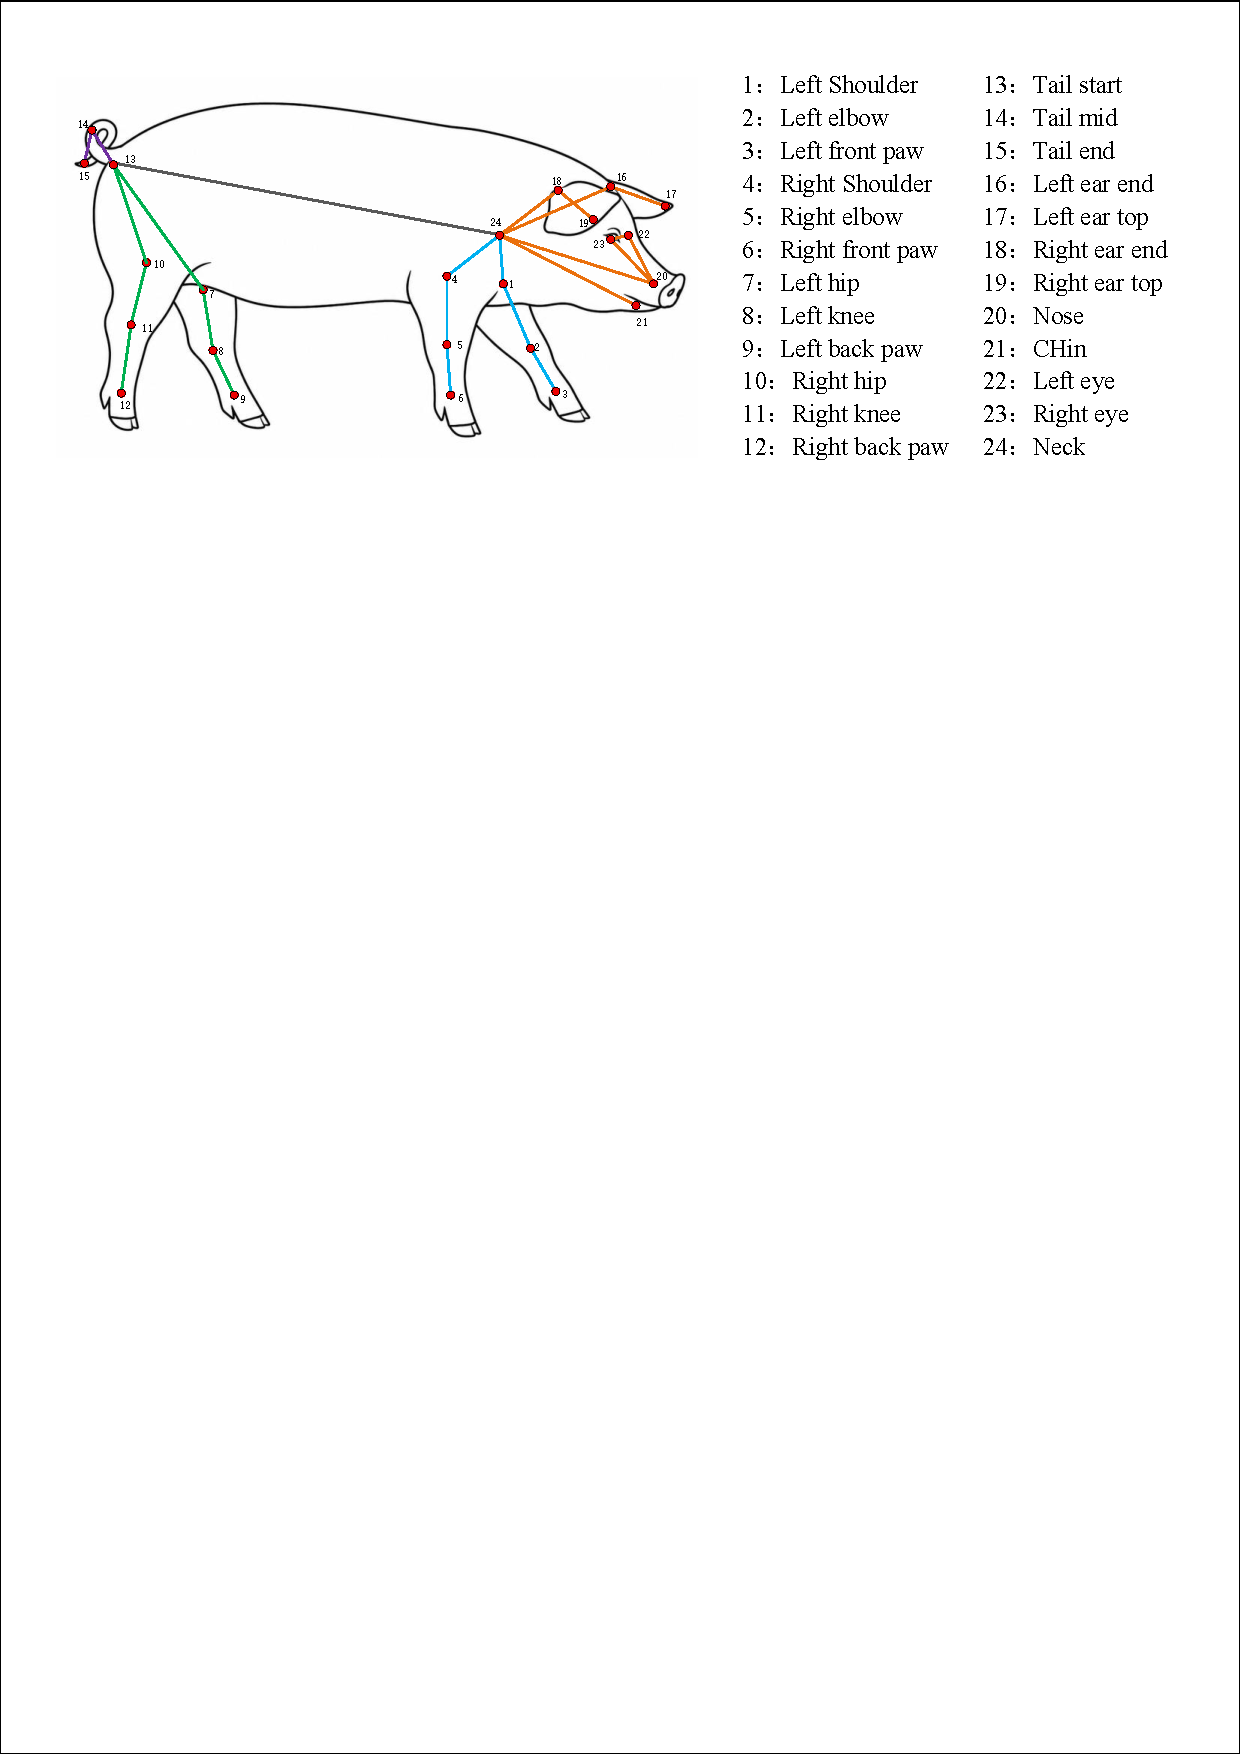
\includegraphics[width=1\textwidth,
trim=1cm 21cm 1cm 1cm,
  clip]{fig/KeyPoint.pdf}

\caption{Pig image annotation examples}
\label{fig:annotation}
\end{figure}

The dataset was randomly divided into training, validation, and test sets with a ratio of 6:3:1, containing 1,625, 812, and 271 images, respectively. Gaussian noise and random channel-brightness adjustment were applied to the training set to improve robustness to poor signals and illumination variations in pig farms. The occlusion-related training and evaluation samples were constructed from the 2,708 annotated images. Natural occlusion samples were retained, and artificial occlusion was further generated by overlaying regular grid-like square blocks on the input images. Specifically, each occlusion block was a black opaque square with a side length of 30 pixels. Adjacent occlusion blocks were separated by 200 pixels in both the horizontal and vertical directions, resulting in a grid step of 230 pixels. The occlusion blocks were periodically arranged from the upper-left corner of the image with the fixed step size. Blocks located near image boundaries were clipped according to the image boundary if they exceeded the image range. According to manual visibility annotations, occluded keypoints accounted for 21.1\% of all annotated keypoints in the dataset, while visible keypoints accounted for 78.9\%, increasing the difficulty of pose estimation and 3D reconstruction.

\subsection{Discrete Latent Pose Completion Module (DLPCM)}
\label{subsec:dlpcm}

DLPCM is not designed as a new standalone 2D pose estimation network. Instead, it is a mask-based keypoint fusion mechanism adapted from neural discrete representation learning for occluded pig pose estimation~\cite{ref28} and integrated into the SMALP reconstruction framework. The original codebook-based occluded pose estimation strategy can infer missing keypoints from visible structural cues, but its predictions for all keypoints may be affected by the capacity and coverage of the learned discrete pose codebook. When the codebook is small or does not sufficiently cover certain pose patterns, visible keypoints that are already reliably detected from the image may also suffer from reconstruction deviations. Therefore, DLPCM uses the discrete latent pose completion result only for occluded keypoints, while visible keypoints are retained from the SMALP keypoint branch.

\begin{figure}
\centering
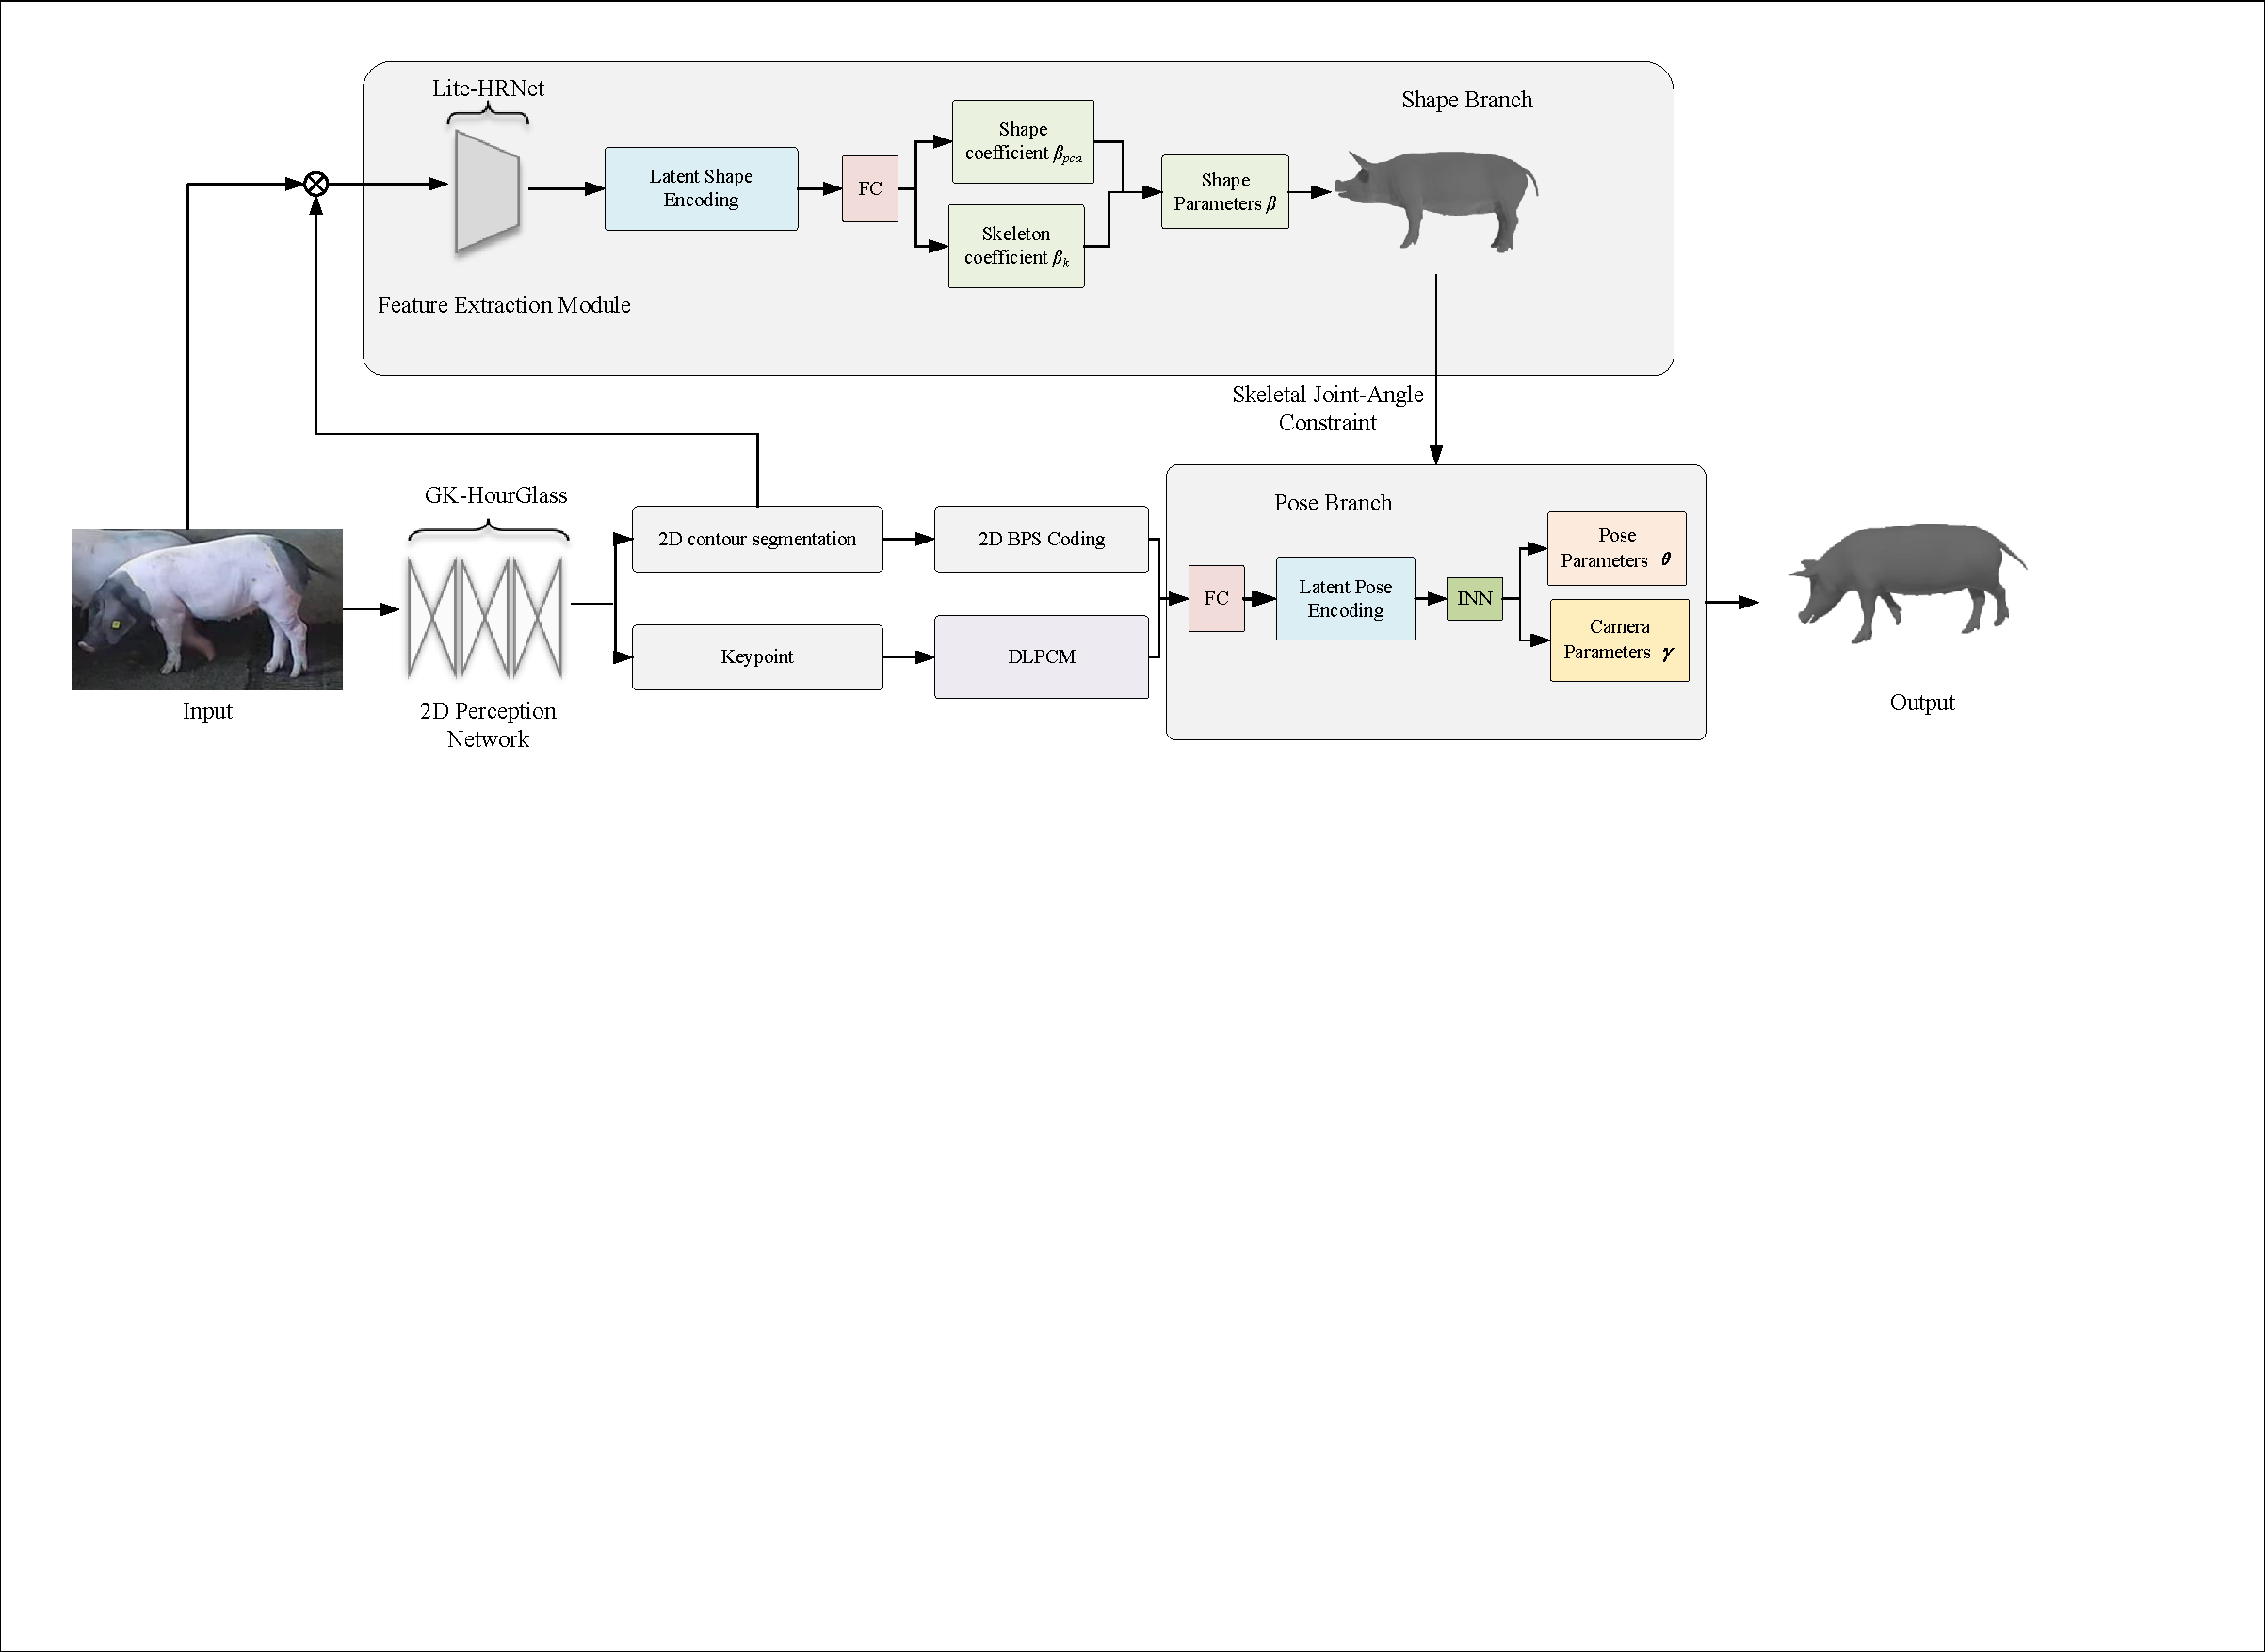
\includegraphics[width=1.2\textwidth,
trim=1cm 16cm 1cm 1cm,
  clip]{fig/fig2.pdf}
\caption{Reconstruction network under occlusion. FC denotes a fully connected layer, and INN denotes an invertible neural network.}
\label{fig:framework}
\end{figure}

First, GK-HourGlass, an improved HourGlass-based keypoint detection backbone, is used to extract features from the input image and simultaneously predict 2D pig keypoint locations and their visibility states. The initial keypoint set is defined as:
\begin{equation}
K_{\text{init}} = \{(x_i, y_i) \mid i = 1, 2, \ldots, N\}
\label{eq:keypoints}
\end{equation}

where $N$ is the number of pig keypoints ($N = 24$).

To distinguish reliable observed keypoints from occluded keypoints, we introduce a keypoint visibility vector automatically predicted by GK-HourGlass:
\begin{equation}
V = \{v_i \mid i = 1, 2, \ldots, N\}
\label{eq:visibility}
\end{equation}

where $v_i$ denotes the predicted visibility of the $i$-th keypoint. When GK-HourGlass predicts the keypoint as visible in the image, $v_i = 1$; when it predicts the keypoint as occluded or invisible, $v_i = 0$.

During pose completion, the input keypoint information $X$ is first fed into an encoder to obtain a continuous latent representation:
\begin{equation}
z_e = E(X)
\label{eq:encoder}
\end{equation}

where $E(\cdot)$ denotes the encoding function. In this work, the codebook size is set to $K = 512$ with codebook-vector dimension $d = 256$.

The encoder output $z_e$ is quantized by nearest-neighbor search:
\begin{equation}
z_q = z_{\arg\min_k \|z_e - z_k\|}
\label{eq:vq}
\end{equation}

where $z_q$ is the quantized discrete latent pose representation.

Then, the decoder predicts the complete keypoint coordinates from the quantized latent vector:
\begin{equation}
K_{\text{comp}} = D(z_q)
\label{eq:decoder}
\end{equation}

To avoid replacing visible keypoints with completion results, the final keypoint set is obtained by mask-based fusion:
\begin{equation}
K_{\text{final}} = M_v \odot K_{\text{init}} + (1 - M_v) \odot K_{\text{comp}}
\label{eq:fusion}
\end{equation}

where $M_v$ denotes the coordinate-level visibility mask, and $\odot$ denotes element-wise multiplication.

\begin{figure}
\centering
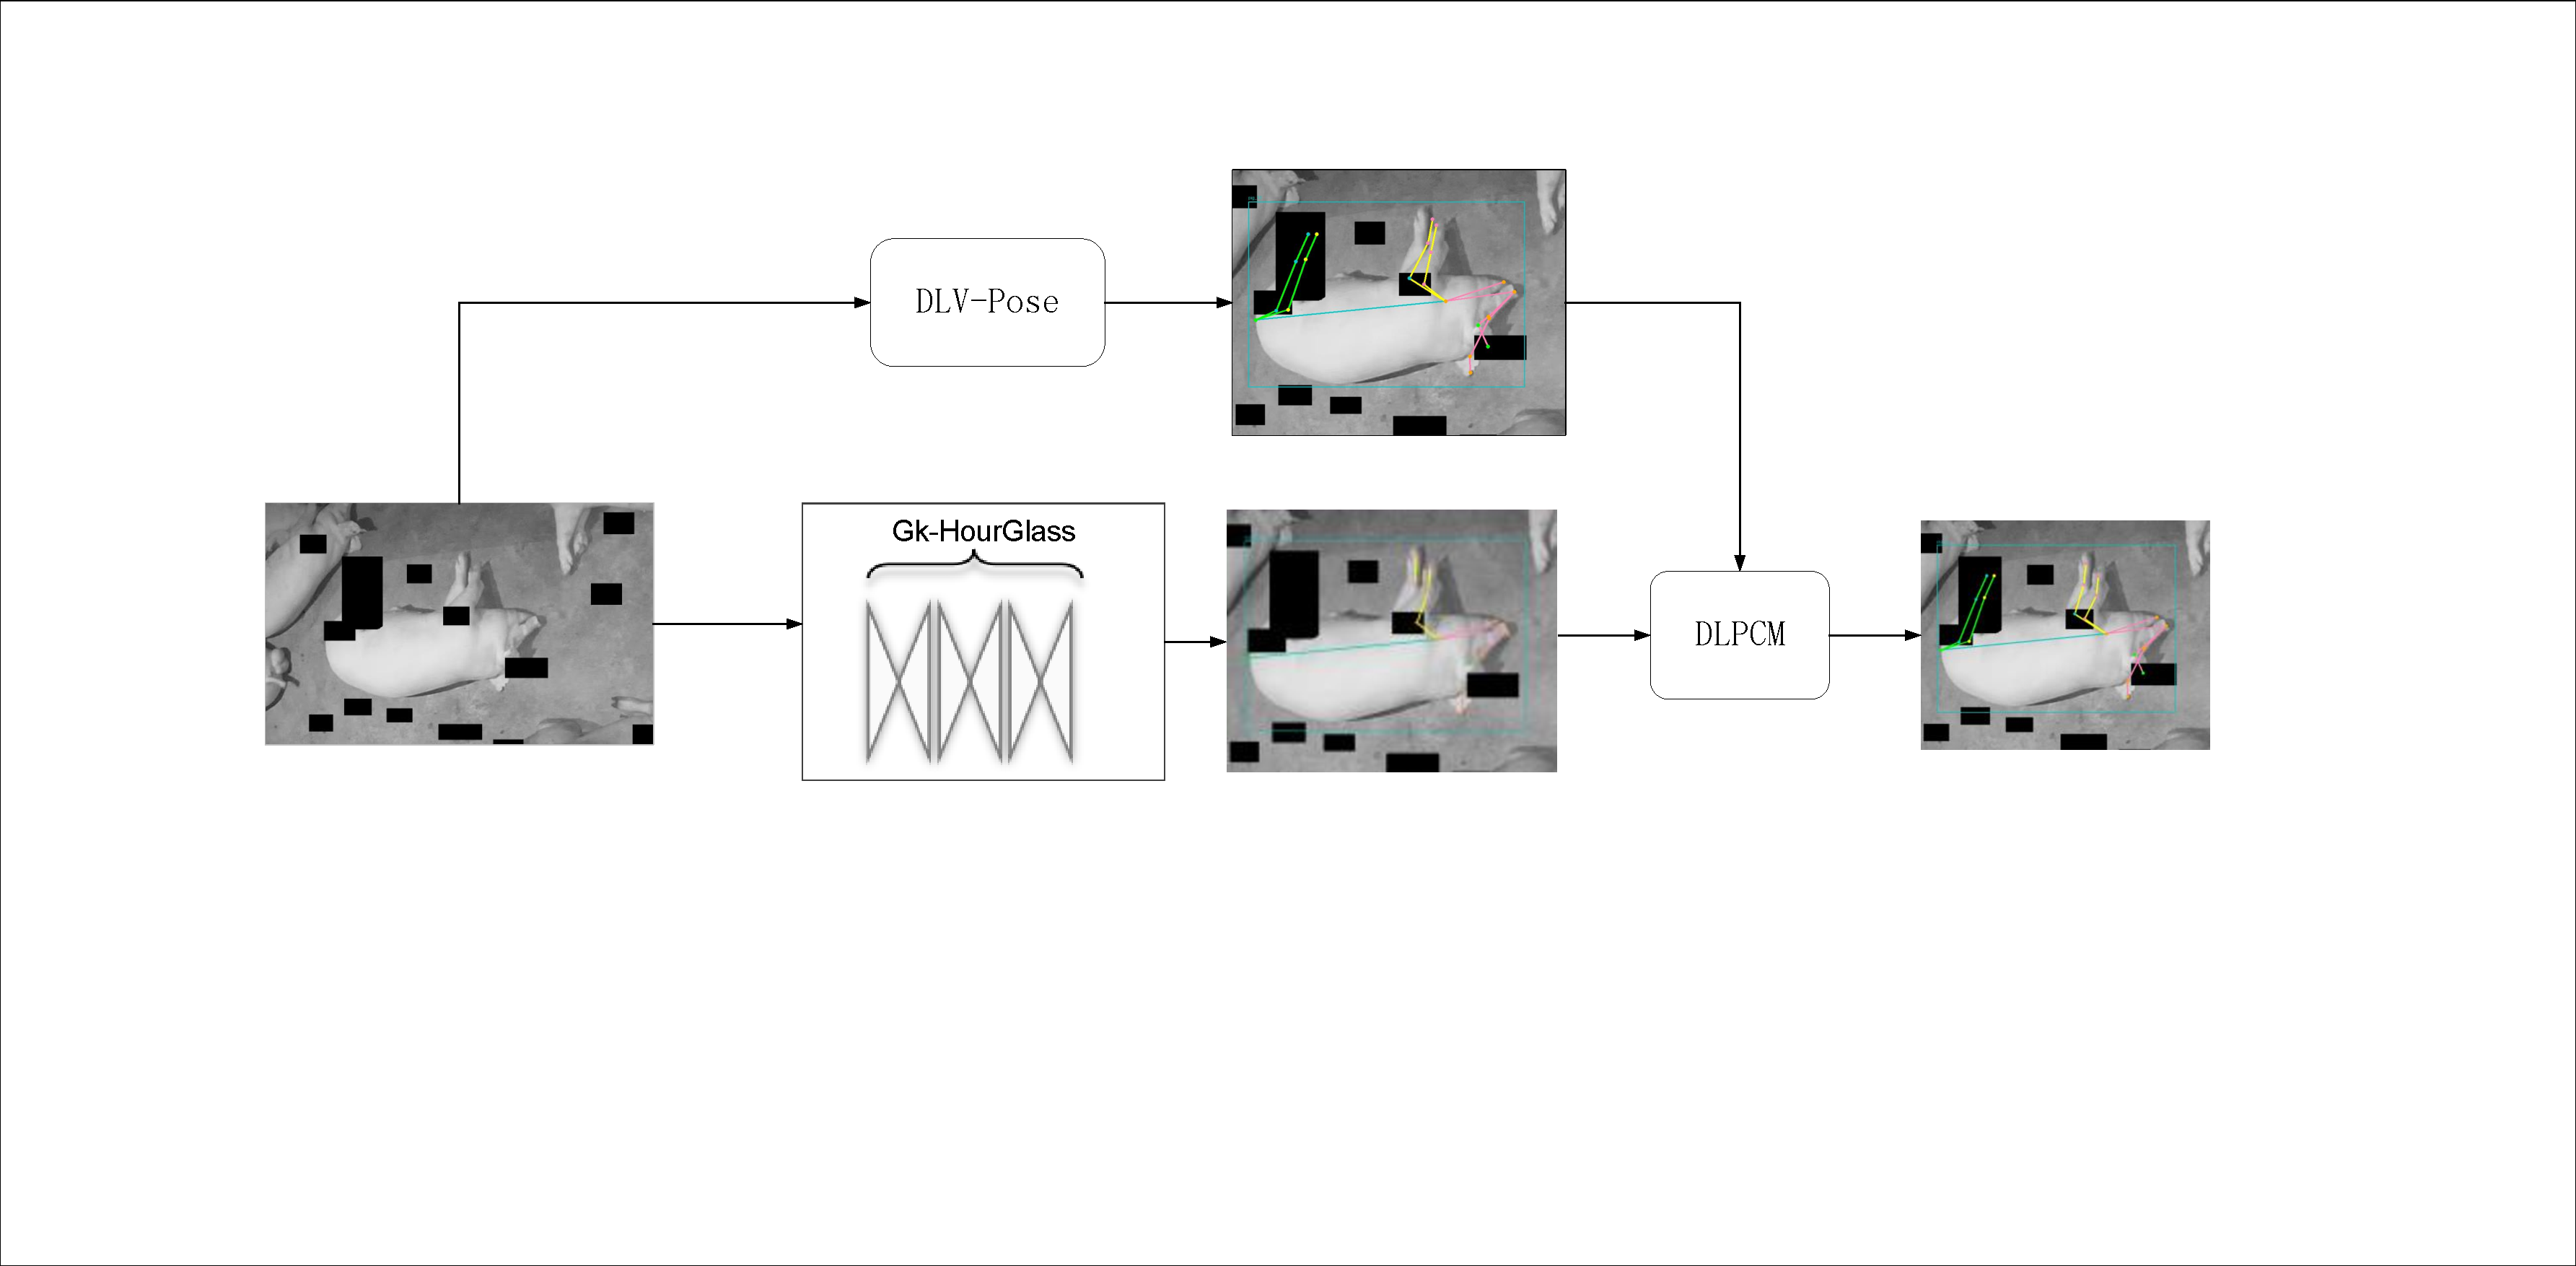
\includegraphics[width=1.1\textwidth,
trim=1cm 11cm 1cm 1cm,
  clip
]{fig/fig3.pdf}
\caption{Mask-based occluded keypoint completion and fusion mechanism. The visibility mask (M$_v$) distinguishes visible keypoints (retained from SMALP) from occluded keypoints (completed by DLPCM).}
\label{fig:dlpcm}
\end{figure}

\subsection{Skeleton-Joint-Angle Constraint (SC)}
\label{subsec:sc}

Although DLPCM can recover partially missing 2D keypoint structures, improved 2D completeness does not necessarily guarantee plausible 3D poses. Under single-view depth ambiguity, local texture loss, and occlusion noise, the pose regressor may still produce backward-bending limbs, excessive local rotations, or twisted leg configurations. To improve pose plausibility under occlusion, we introduce a Skeleton-joint-angle constraint (SC) in the pose-parameter regression stage.

SC specifically denotes a Skeleton-joint-angle constraint on local joint rotations. It does not contain any bone-length constraint or skeletal-scale constraint. Inter-individual differences in body shape and skeletal proportion are represented by the SMALP shape parameters, and no additional fixed constraint is imposed on bone lengths. Therefore, SC focuses on suppressing abnormal local rotations in the pose-parameter space rather than restricting natural body-shape variation among pigs.

Since limb joints have larger motion freedom than the torso and are more vulnerable to occlusion-induced errors, the constraint is mainly applied to major limb joints, including the shoulder, elbow, hip, and knee joints. These joints exhibit the largest range of motion during pig locomotion and are most susceptible to occlusion-induced errors, making them critical targets for pose plausibility constraints.

For each constrained joint $j$, the constraint is defined as:
\begin{equation}
\mathcal{L}_{\text{SC}} = \sum_{j \in \mathcal{J}} \max(0, a_j - a_j^{\max})^2
\label{eq:sc_loss}
\end{equation}

where $a_j$ denotes the local rotation magnitude of the $j$-th joint, and $a_j^{\max}$ is the maximum allowed angle.

Based on gait analysis and biomechanical studies of pigs and similar quadrupeds~\cite{ref29,ref30,ref31}, typical joint angle ranges during normal locomotion are:

\begin{itemize}
\item Knee joint (stifle): Flexion range 0°--120°, typical active range during gait 20°--80°
\item Elbow joint: Flexion range 0°--110°, typical active range during gait 15°--70°
\item Hip joint: Flexion range 0°--150°, typical active range during gait 30°--90°
\item Shoulder joint: Flexion range 0°--140°, typical active range during gait 20°--100°
\end{itemize}

\subsection{Training Strategy and Loss Function}
\label{subsec:training}

The training procedure consists of two stages. In Stage 1, we train the 2D keypoint modules, including the SMALP keypoint branch and DLPCM for occluded keypoint completion. In Stage 2, the trained 2D modules are integrated into SMALP. DLPCM performs mask-based fusion by retaining visible keypoints predicted by the SMALP keypoint branch and replacing only occluded keypoints with the completion results.

The 3D reconstruction network is optimized under a weakly supervised objective with keypoint projection consistency, silhouette consistency, and shape/pose regularization. With the skeleton-joint-angle constraint (SC), the 3D loss is:
\begin{equation}
L_{3D} = L_{\text{rec}} + \lambda_s L_{\text{SC}}
\label{eq:3d_loss}
\end{equation}

where $L_{\text{rec}}$ denotes the basic weakly supervised reconstruction loss and $L_{\text{SC}}$ denotes the skeleton-joint-angle penalty. $\lambda_s$ is the weight of SC.

\section{Results and Analysis}
\label{sec:results}

To verify the effectiveness of the proposed method, the experiments are organized in a progressive manner. First, 2D occluded keypoint prediction experiments are used to evaluate whether DLPCM can provide more reliable keypoint estimates under occlusion. Second, 3D reconstruction ablation experiments are conducted to analyze whether the completed occluded keypoints improve SMALP reconstruction. Finally, the effect of SC is evaluated from pose-parameter plausibility and qualitative visualization. Since dense 3D ground truth is unavailable in real pig-farm images, the 3D reconstruction results are interpreted mainly from 2D projection consistency, silhouette consistency, and pose plausibility.

\subsection{2D Occluded Keypoint Prediction Experiment}
\label{subsec:2d_results}

To evaluate the effectiveness of the discrete latent pose completion strategy adopted by DLPCM, pig images containing occlusion were used as the test set. This experiment focuses on the 2D stage and verifies whether codebook-based latent pose completion can provide more reliable estimates for occluded keypoints. The traditional heatmap-based prediction strategy and the DLPCM-assisted prediction strategy were compared under different backbone networks. The occlusion types mainly included limb self-occlusion, inter-individual occlusion, and fence occlusion. HourGlass, Stacked-HourGlass, HR-Former, and GK-HourGlass were selected as backbones to evaluate the adaptability of DLPCM to different network structures.

Keypoint prediction performance was evaluated using AP, AP50, AP75, AP(S), AP(M), and AP(L). AP denotes average precision for keypoints. AP50 and AP75 denote keypoint detection precision under different OKS thresholds, and AP(S), AP(M), and AP(L) denote keypoint prediction precision for small, medium, and large targets, respectively.

\begin{table}
\centering
\caption{2D keypoint prediction results of DLPCM-assisted and heatmap-based strategies on the occluded pig test set}
\label{tab:2d_results}
\begin{tabular}{lccccc}
\toprule
Method & AP & AP50 & AP75 & AP(M) & AP(L) \\
\midrule
HourGlass (baseline) & 33.2 & 45.8 & 23.3 & 35.4 & 40.9 \\
HourGlass + DLPCM & 37.9 & 52.1 & 31.8 & 40.2 & 47.8 \\
GK-HourGlass (baseline) & 37.9 & 51.2 & 28.5 & 40.1 & 47.3 \\
GK-HourGlass + DLPCM & 42.2 & 56.8 & 35.9 & 44.8 & 50.8 \\
\bottomrule
\end{tabular}
\end{table}

As shown in Table~\ref{tab:2d_results}, the DLPCM-assisted strategy achieves higher keypoint prediction accuracy than the traditional heatmap-based strategy on all four backbones. Taking HourGlass as an example, the DLPCM-assisted strategy improves AP from 33.2 to 37.9 and AP75 from 23.3 to 31.8, indicating a more obvious improvement in high-precision keypoint localization. For the stronger GK-HourGlass backbone, the DLPCM-assisted strategy still improves AP from 37.9 to 42.2, demonstrating good adaptability to different network architectures.

\subsection{3D Reconstruction Ablation Study}
\label{subsec:3d_ablation}

To verify the effects of DLPCM and SC on single-view 3D pig reconstruction, four ablation settings were designed. The baseline corresponds to the weakly supervised SMALP reconstruction network without DLPCM or SC. The other settings include baseline with only DLPCM, baseline with only SC, and baseline with both DLPCM and SC.

\begin{table}
\centering
\caption{Ablation study results: Effects of DLPCM and SC on 3D pig reconstruction}
\label{tab:ablation}
\begin{tabular}{lccc}
\toprule
Method & PCK@0.1 (\%) & IoU (\%) & JRVR (\%) \\
\midrule
Baseline & 61.85 & 64.04 & 69.74 \\
Baseline + DLPCM & 66.73 & 67.90 & 24.34 \\
Baseline + SC & 64.79 & 66.32 & 12.50 \\
Baseline + DLPCM + SC & 64.91 & 66.05 & 9.38 \\
\bottomrule
\end{tabular}
\end{table}

As shown in Table~\ref{tab:ablation}, DLPCM improves PCK from 61.85\% to 66.73\% and IoU from 64.04\% to 67.90\%, while reducing JRVR from 69.74\% to 24.34\%. SC further reduces abnormal local rotations, achieving the lowest JRVR of 9.38\% while maintaining competitive PCK and IoU. These results indicate that DLPCM mainly improves occluded structural observations, whereas SC improves pose plausibility, leading to a better trade-off between projection consistency and pose plausibility under occlusion.

\subsection{Visualization Analysis of Reconstruction Results}
\label{subsec:visualization}

To verify the adaptability of the proposed method in complex farming environments, three typical occlusion scenarios were selected for visualization analysis: pig self-occlusion, occlusion by other pigs, and fence occlusion.

\begin{figure}
\centering
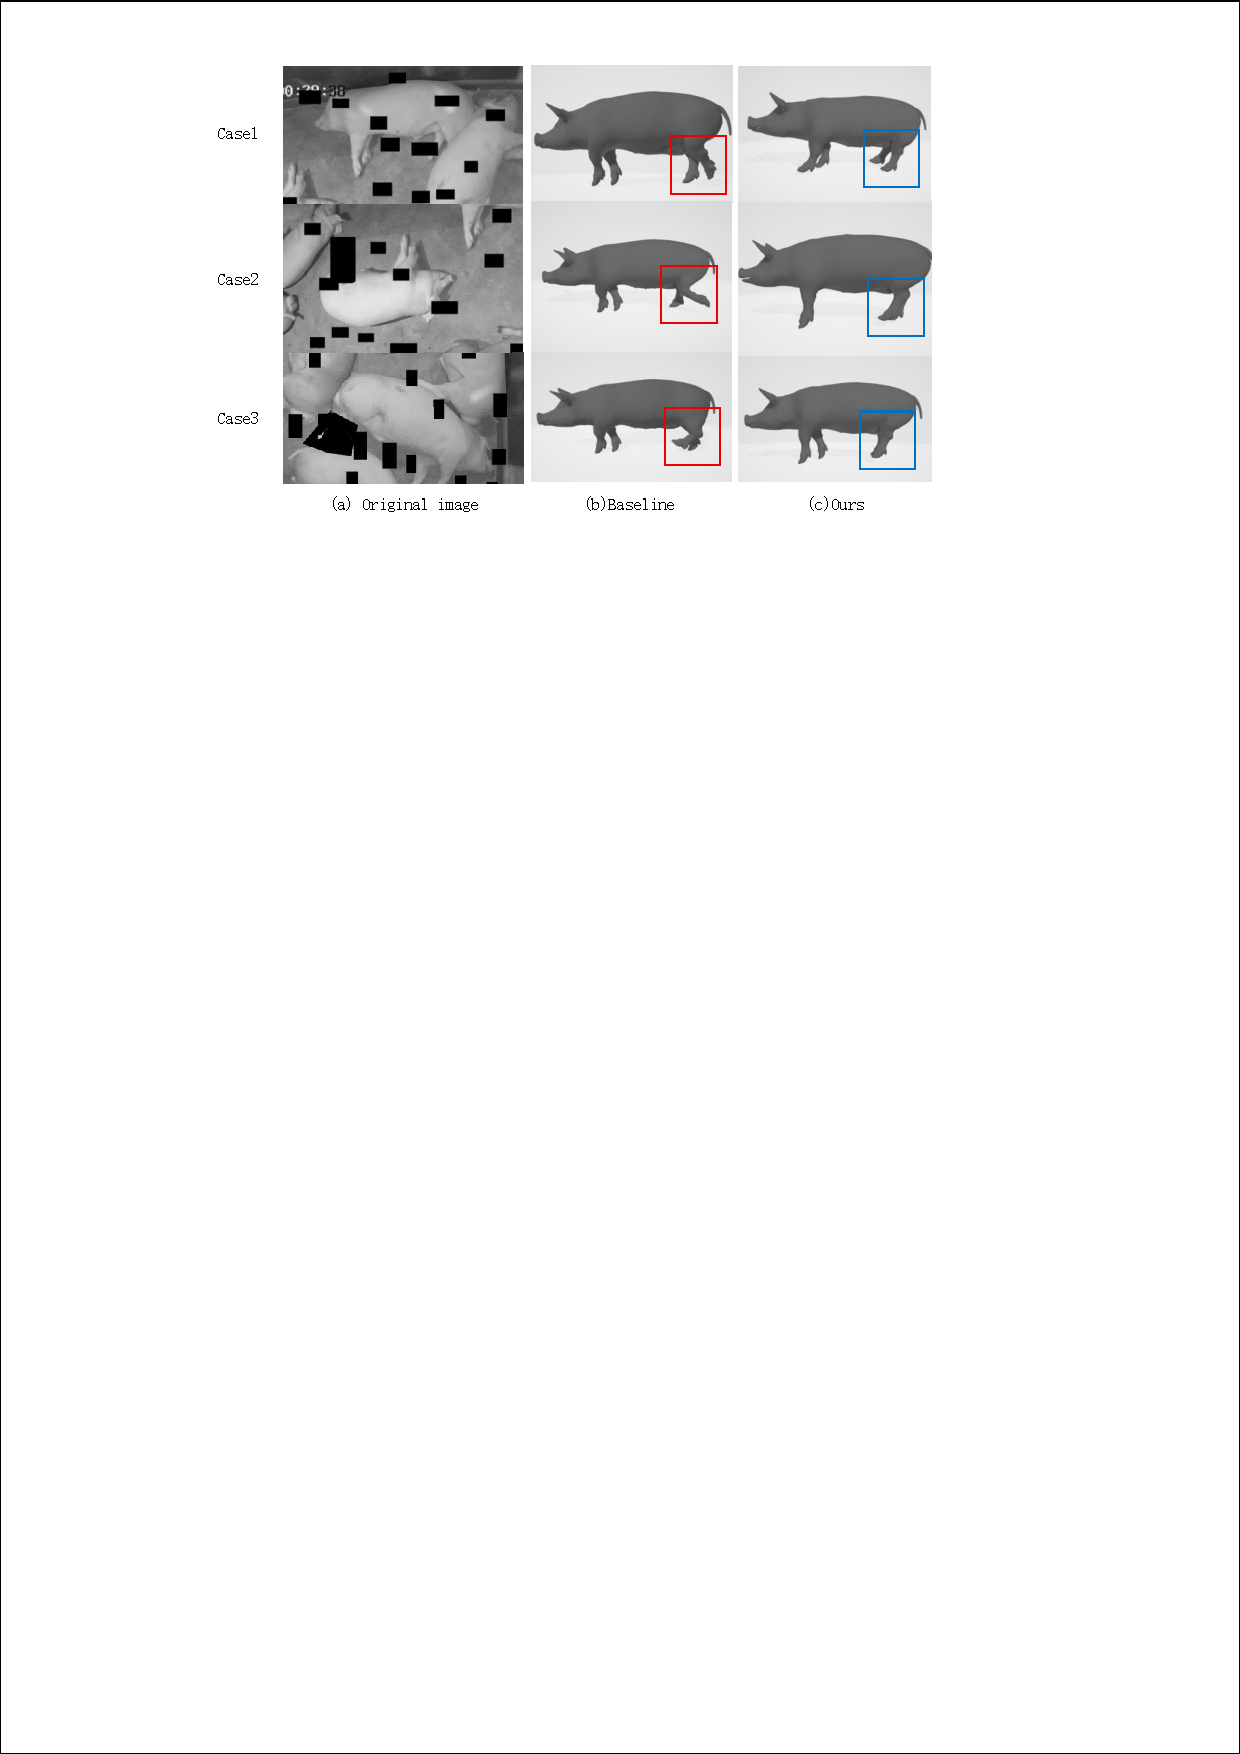
\includegraphics[width=0.9\textwidth]{fig/DLPCM.pdf}
\caption{3D pose reconstruction of pigs under occlusion. (a) Pig self-occlusion. (b) Occlusion by other pigs. (c) Fence occlusion. The proposed method recovers continuous 3D poses with fewer backward-bending or local-twisting artifacts compared to baseline.}
\label{fig:occlusion}
\end{figure}

As shown in Fig.~\ref{fig:occlusion}, the proposed method can recover relatively continuous 3D pig poses under the three occlusion scenarios. In particular, in the leg-joint regions, the model produces fewer obvious backward-bending or local-twisting artifacts, indicating that occluded keypoint completion and the Skeleton-joint-angle constraint improve pose plausibility under complex occlusion.

To further observe the performance of the method under severe local occlusion, artificial occlusion was added to test images, mainly covering the leg-joint regions so that some leg keypoints became invisible. To verify the effect of DLPCM on 3D pig reconstruction, the same pig image was reconstructed using the original SMALP reconstruction network and the SMALP network integrated with DLPCM. The reconstruction results are shown in Fig.~\ref{fig:dlpcm_effect}.

\begin{figure}
\centering
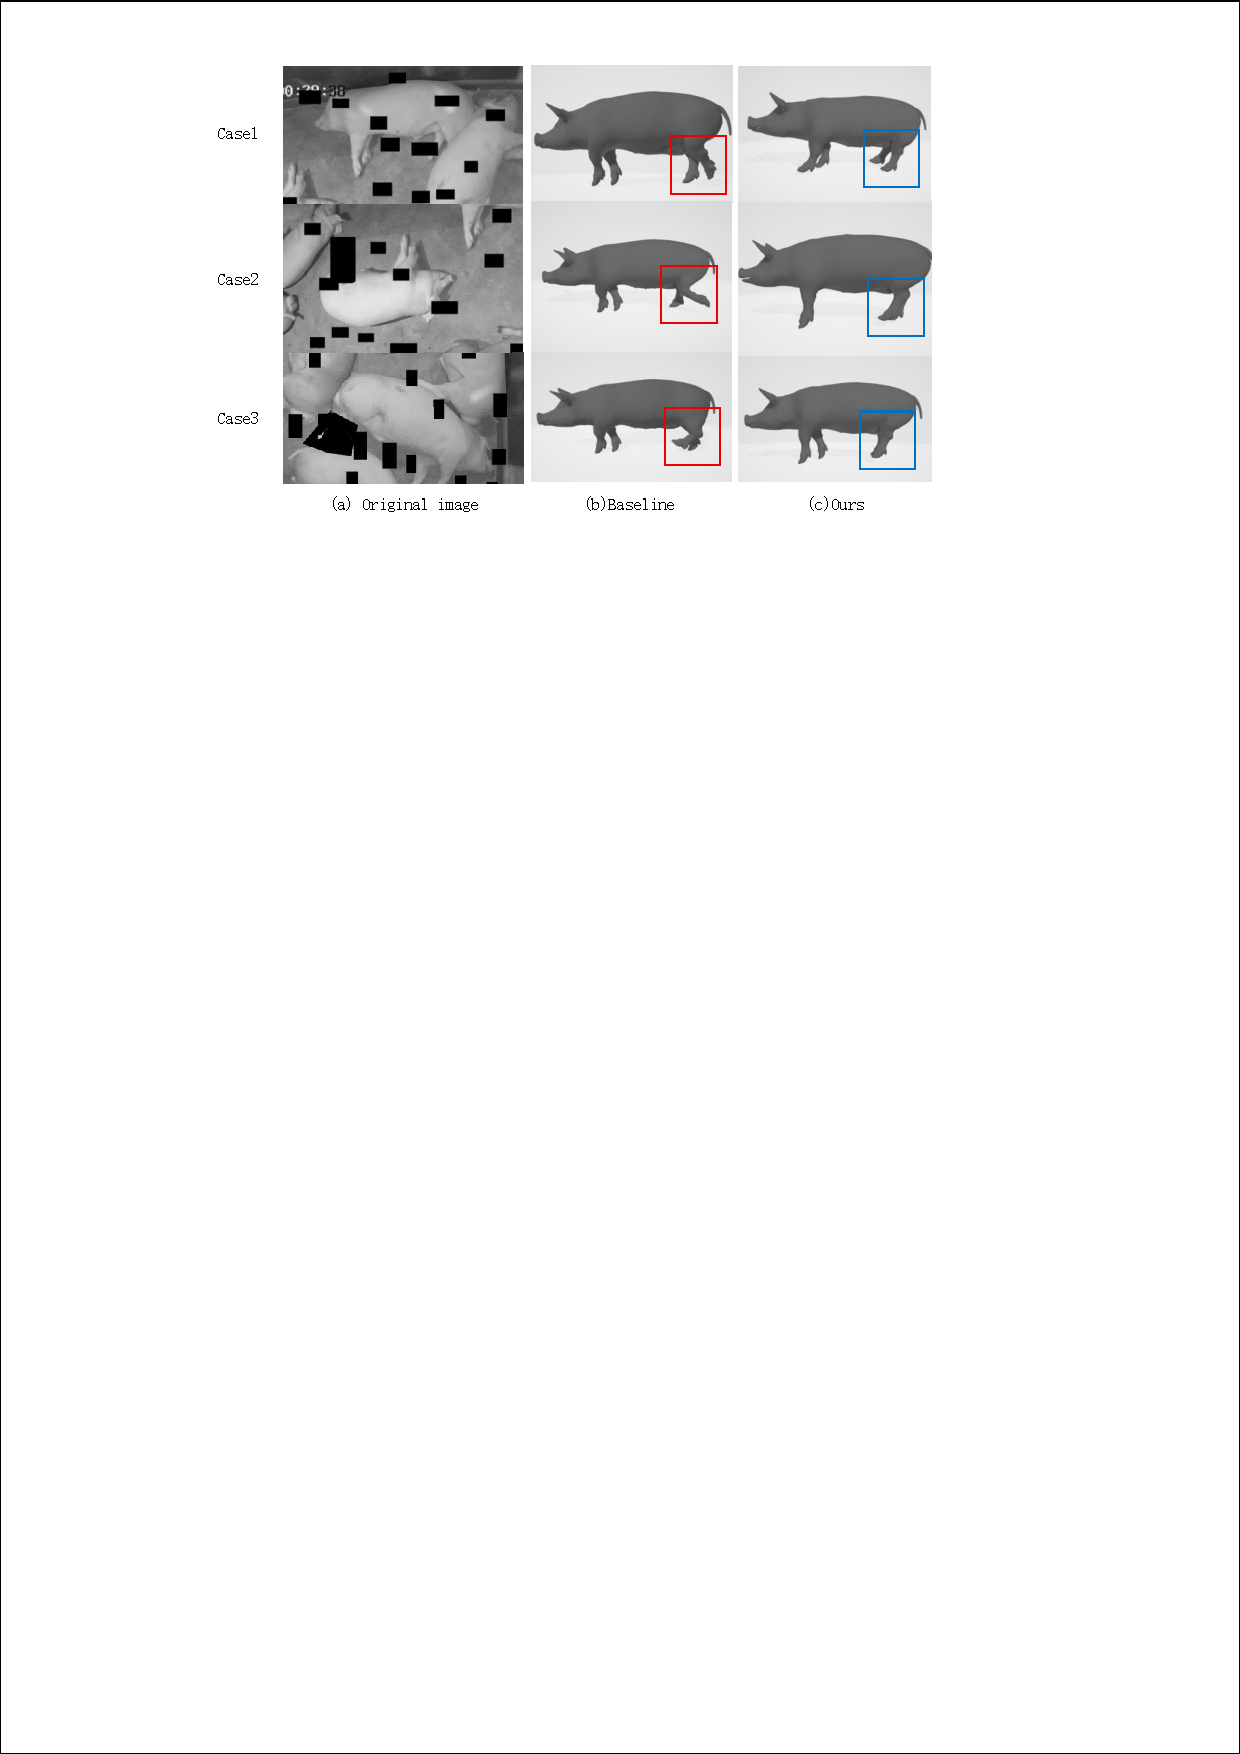
\includegraphics[width=1.1\textwidth,trim=3cm 21cm 3cm 1cm, clip]{fig/DLPCM.pdf}
\caption{3D reconstruction incorporating DLPCM. (a) Original image. (b) Reconstruction result of the baseline SMALP model without DLPCM, showing joint-position deviations in occluded leg regions. (c) Reconstruction result after incorporating DLPCM, with more continuous leg joints. Visible keypoints are retained from the SMALP keypoint branch, while occluded keypoints are completed by DLPCM.}
\label{fig:dlpcm_effect}
\end{figure}

As shown in Fig.~\ref{fig:dlpcm_effect}, when processing samples with occluded legs, the original SMALP reconstruction network tends to produce joint-position deviations and local pose distortions due to insufficient 2D observations. After incorporating DLPCM, the model can infer the 2D positions of occluded body parts based on the structural relationships among visible keypoints, making the recovered leg joints more continuous. This suggests that DLPCM provides more stable 2D structural constraints for subsequent 3D pose regression.


\begin{figure}
\centering
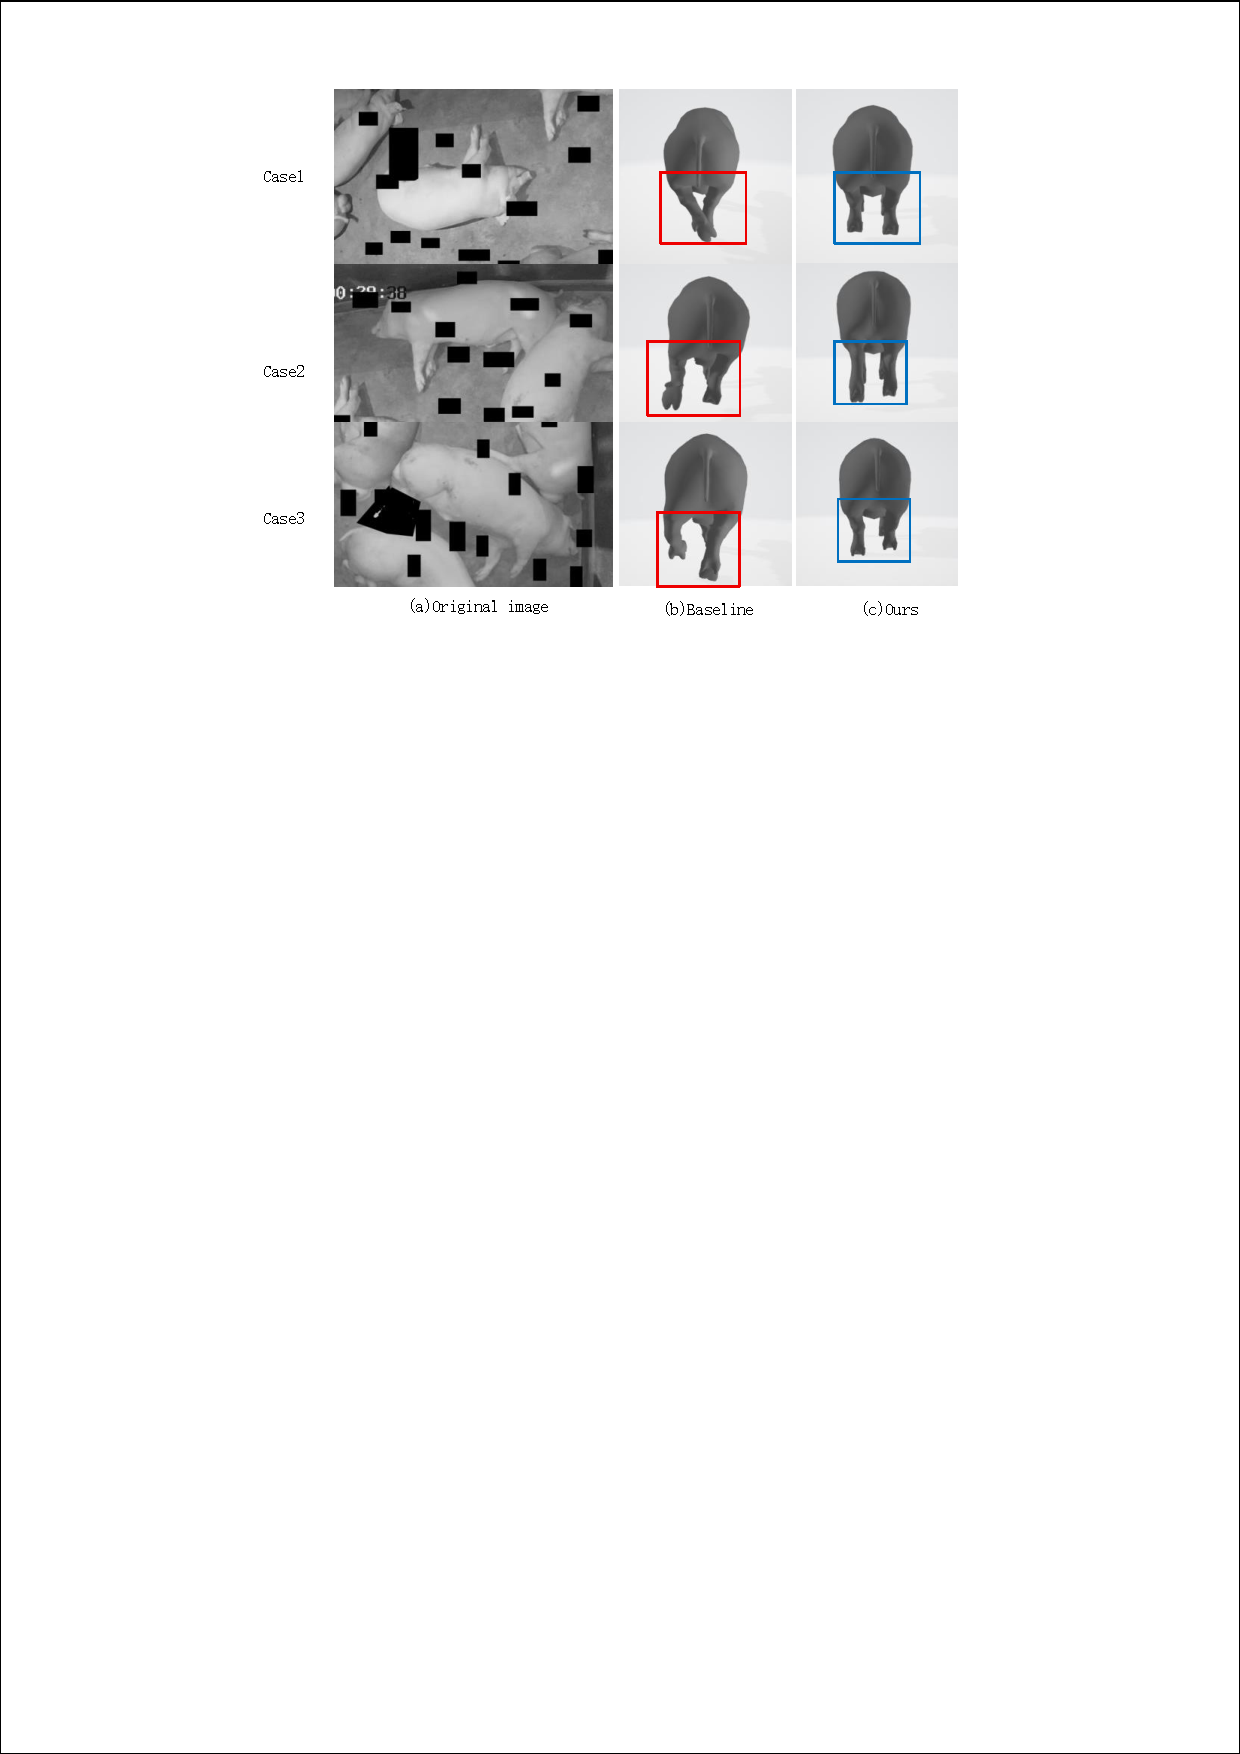
\includegraphics[width=1.3\textwidth,trim=4cm 18cm 1cm 1cm, clip]{fig/sc.pdf}
\caption{3D reconstruction of pig pose with the Skeleton-joint-angle constraint (SC). Compared with unconstrained results, SC restricts abnormal rotations of major leg joints (hip, knee) and reduces distorted regions to plausible poses.}
\label{fig:sc_effect}
\end{figure}
Fig.~\ref{fig:sc_effect} shows the 3D reconstruction results after adding the Skeleton-joint-angle constraint. Compared with the unconstrained result, SC restricts abnormal rotations of major leg joints such as the hip and knee joints and makes distorted regions closer to plausible poses. This further indicates that the main function of SC is not simply to improve 2D projection metrics but to reduce abnormal local rotation patterns in the pose-parameter space.

\begin{figure}
\centering
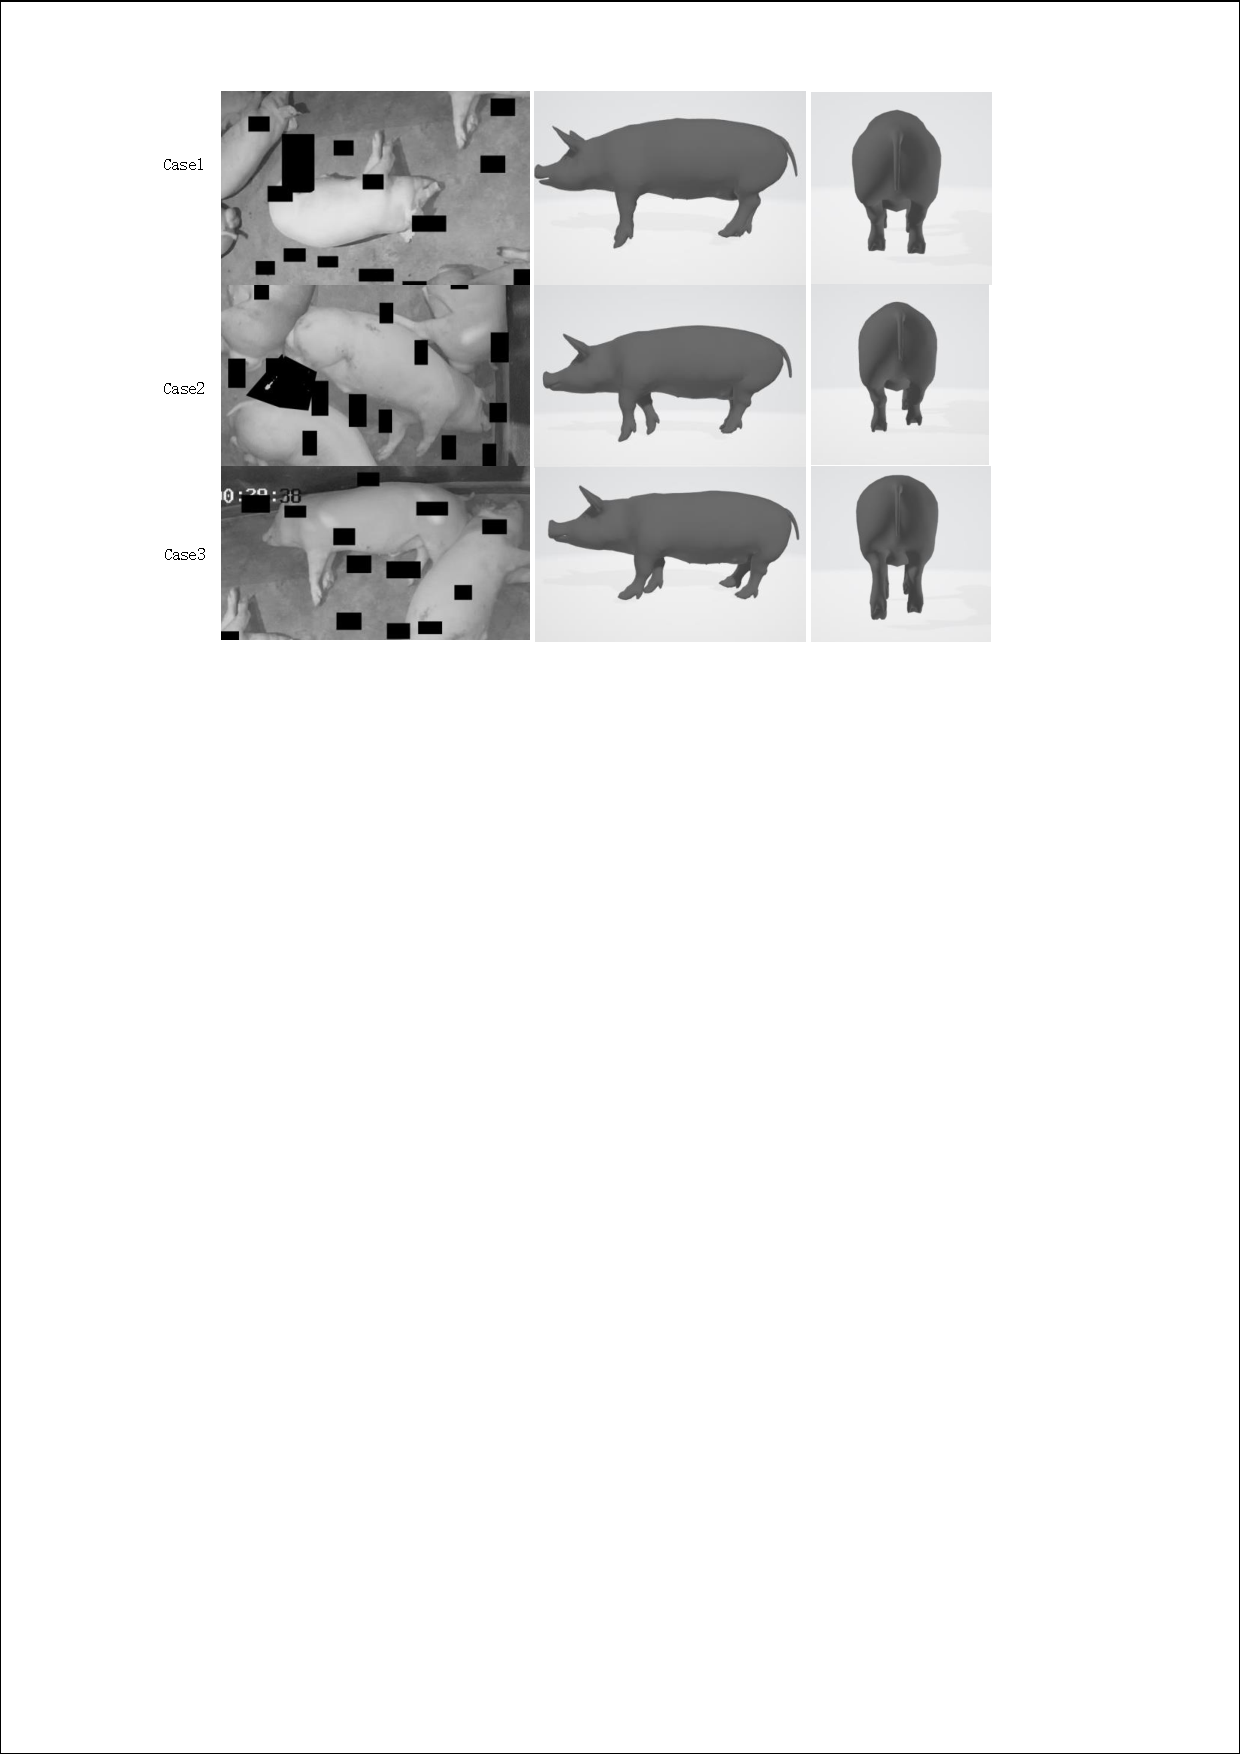
\includegraphics[width=1.1\textwidth,trim=1cm 18cm 1cm 1cm, clip]{fig/DLCPM+SC.pdf}
\caption{Multi-view visualization of 3D pig pose reconstruction with the Skeleton-joint-angle constraint. (a) Original image. (b) Side view showing plausible limb configurations. (c) Rear view demonstrating pose stability under occlusion.}
\label{fig:multiview}
\end{figure}

The results in Fig.~\ref{fig:multiview} show that the proposed method can recover relatively plausible 3D pig poses even when image information is incomplete. Combined with the quantitative experiments, DLPCM mainly improves structural observations in occluded regions, while SC mainly reduces abnormal joint rotations. Together, they improve pose stability for single-view 3D pig reconstruction in complex farming environments.

\section{Limitations and Future Work}
\label{sec:limitations}

The Skeleton-joint-angle constraint thresholds are empirically set based on the current pig dataset and may require adjustment for other pig breeds, ages, or body conditions. The generalization of SC to diverse pig populations and its transferability across different farming environments require further validation.

Future work could explore: (1) extending to multi-pig scenarios, (2) improving real-time performance, (3) incorporating temporal information for video-based reconstruction.

\section{Conclusion}
\label{sec:conclusion}

This paper addresses the challenge of occluded pig pose estimation in real-world farming environments. We propose an occlusion-stable single-view 3D pig reconstruction framework that integrates a mask-based keypoint fusion mechanism (DLPCM) and a Skeleton-joint-angle constraint (SC). Experimental results demonstrate significant improvements in both 2D keypoint prediction and 3D pose reconstruction under occlusion. DLPCM improves PCK and IoU while SC improves pose plausibility, leading to a better trade-off between projection consistency and pose plausibility under occlusion.

\begin{credits}
\subsubsection{\ackname}
This study was funded by the Key Laboratory of Smart Farming Technology, Ministry of Agriculture and Rural Affairs.

\subsubsection{\discintname}
The authors have no competing interests to declare that are relevant to the content of this article.
\end{credits}

\begin{thebibliography}{99}

\bibitem{ref1}
Li, B.M., Wang, Y., Zheng, W.C., et al.: Research progress on intelligent equipment and information technology for livestock and poultry farming. Journal of South China Agricultural University \textbf{42}(6), 1--15 (2021). \url{https://doi.org/10.7671/j.issn.1671-9352.2021.06.001}

\bibitem{ref2}
Yang, L., Wang, H., Chen, R.P., et al.: Research progress of intelligent pig farming factories. Journal of South China Agricultural University \textbf{44}(2), 1--12 (2023). \url{https://doi.org/10.7671/j.issn.1671-9352.2023.02.001}

\bibitem{ref3}
Guo, Y.Y., Du, S.Z., Qiao, Y.L., et al.: Research and application progress of deep learning in intelligent livestock farming. Smart Agriculture \textbf{5}(1), 1--18 (2023). \url{https://doi.org/10.12133/j.smartag.2023.5.1.202209-00001}

\bibitem{ref4}
Zhang, J.L., Zhuang, Y.R., Zhou, K., et al.: Design and experiment of a fattening pig grouping system based on machine vision. Transactions of the Chinese Society of Agricultural Engineering \textbf{36}(17), 196--203 (2020). \url{https://doi.org/10.11975/j.issn.1002-6819.2020.17.023}

\bibitem{ref5}
Yao, Y.P., Xu, C., Chen, H.J., et al.: Pig body-size estimation based on keypoint detection and multi-object tracking. Journal of South China Agricultural University \textbf{45}(5), 722--729 (2024). \url{https://doi.org/10.7671/j.issn.1671-9352.2024.05.013}

\bibitem{ref6}
Hu, Z.X., Xiang, L., Yang, B., et al.: Multi-view voxel-based 3D skeleton reconstruction for pig lameness detection. Transactions of the Chinese Society of Agricultural Engineering \textbf{45}(5), 703--715 (2024). \url{https://doi.org/10.11975/j.issn.1002-6819.2024.05.078}

\bibitem{ref7}
Liu, L.S., Liu, L., Zhou, J., et al.: Research progress on intelligent perception technologies for precision sow farming. Journal of South China Agricultural University \textbf{45}(5), 690--702 (2024). \url{https://doi.org/10.7671/j.issn.1671-9352.2024.05.012}

\bibitem{ref8}
Zhao, C.J., Li, D.L., Liu, G., et al.: Research on the development status and strategic objectives of smart agriculture. Strategic Study of CAE \textbf{20}(2), 1--8 (2018). \url{https://doi.org/10.15302/J-SSCAE-2018.02.001}

\bibitem{ref9}
Qin, C.Y., Chen, M., Zhang, M., et al.: Research progress on the application of computer vision technology in modern agriculture. Journal of Chinese Agricultural Mechanization \textbf{44}(12), 160--170 (2023). \url{https://doi.org/10.13733/j.jcam.issn.2095-5553.2023.12.025}

\bibitem{ref10}
Wang, C., Zhang, M., Li, H., et al.: Research progress on automatic measurement technology of livestock body size. Transactions of the Chinese Society of Agricultural Engineering \textbf{38}(13), 255--268 (2022). \url{https://doi.org/10.11975/j.issn.1002-6819.2022.13.029}

\bibitem{ref11}
Liang, J., Yuan, Z., Luo, X., et al.: A study on the 3D reconstruction strategy of a sheep body based on a Kinect v2 depth camera array. Animals \textbf{14}(17), 2457 (2024). \url{https://doi.org/10.3390/ani14172457}

\bibitem{ref12}
Qi, C.R., Yi, L., Su, H., et al.: PointNet++: Deep hierarchical feature learning on point sets in a metric space. In: Proceedings of the 31st International Conference on Neural Information Processing Systems, pp. 5105--5114 (2017). \url{https://arxiv.org/abs/1706.02413}

\bibitem{ref13}
Hao, H., Yang, J., Yin, L., et al.: An improved PointNet++ point cloud segmentation model applied to automatic measurement method of pig body size. Computers and Electronics in Agriculture \textbf{205}, 107560 (2023). \url{https://doi.org/10.1016/j.compag.2023.107560}

\bibitem{ref14}
Jiang, Y., Li, Z., Cao, J., et al.: Body parts segmentation and phenotypic trait extraction of pig using an improved point cloud segmentation network with multi-LiDAR. Computers and Electronics in Agriculture \textbf{237}, 110624 (2025). \url{https://doi.org/10.1016/j.compag.2024.110624}

\bibitem{ref15}
Nath, T., Mathis, A., Chen, A.C., et al.: Using DeepLabCut for 3D markerless pose estimation across species and behaviors. Nature Protocols \textbf{14}, 2152--2176 (2019). \url{https://doi.org/10.1038/s41596-019-0176-0}

\bibitem{ref16}
Karashchuk, P., Rupp, K.L., Dickinson, E.S., et al.: Anipose: A toolkit for stable markerless 3D pose estimation. Cell Reports \textbf{36}(13), 109730 (2021). \url{https://doi.org/10.1016/j.celrep.2021.109730}

\bibitem{ref17}
Waldmann, U., Chan, A.H.H., Naik, H., et al.: 3D-MuPPET: 3D multi-pigeon pose estimation and tracking. International Journal of Computer Vision \textbf{132}, 4235--4252 (2024). \url{https://doi.org/10.1007/s11263-024-02024-6}

\bibitem{ref18}
An, L., Ren, J., Yu, T., et al.: Three-dimensional surface motion capture of multiple freely moving pigs using MAMMAL. Nature Communications \textbf{14}, 7727 (2023). \url{https://doi.org/10.1038/s41467-023-43343-7}

\bibitem{ref19}
Loper, M., Mahmood, N., Romero, J., et al.: SMPL: A skinned multi-person linear model. ACM Transactions on Graphics \textbf{34}(6), 248 (2015). \url{https://doi.org/10.1145/2816795.2818013}

\bibitem{ref20}
Zuffi, S., Kanazawa, A., Jacobs, D.W., et al.: 3D Menagerie: Modeling the 3D shape and pose of animals. In: Proceedings of the IEEE Conference on Computer Vision and Pattern Recognition, pp. 6365--6373 (2017). \url{https://doi.org/10.1109/CVPR.2017.674}

\bibitem{ref21}
Zuffi, S., Kanazawa, A., Black, M.J.: Lions and tigers and bears: Capturing non-rigid, 3D, articulated shape from images. In: Proceedings of the IEEE Conference on Computer Vision and Pattern Recognition, pp. 3955--3963 (2018). \url{https://doi.org/10.1109/CVPR.2018.00416}

\bibitem{ref22}
Zuffi, S., Kanazawa, A., Berger-Wolf, T., et al.: Three-D Safari: Learning to estimate zebra pose, shape, and texture from images in the wild. In: Proceedings of the IEEE/CVF International Conference on Computer Vision, pp. 5359--5368 (2019). \url{https://doi.org/10.1109/ICCV.2019.00546}

\bibitem{ref23}
Biggs, B., Boyne, O., Charles, J., et al.: Who left the dogs out? 3D animal reconstruction with expectation maximization in the loop. In: European Conference on Computer Vision, pp. 195--211 (2020). \url{https://doi.org/10.1007/978-3-030-58580-8_12}

\bibitem{ref24}
Li, C., Lee, G.H.: Coarse-to-fine animal pose and shape estimation. In: Advances in Neural Information Processing Systems, vol. 34, pp. 11757--11768 (2021). \url{https://arxiv.org/abs/2109.07378}

\bibitem{ref25}
Rüegg, N., Zuffi, S., Schindler, K., et al.: BARC: Learning to regress 3D dog shape from images by exploiting breed information. In: Proceedings of the IEEE/CVF Conference on Computer Vision and Pattern Recognition, pp. 3876--3884 (2022). \url{https://doi.org/10.1109/CVPR52688.2022.00385}

\bibitem{ref26}
Rüegg, N., Tripathi, S., Schindler, K., et al.: BITE: Beyond priors for improved three-D dog pose estimation. In: Proceedings of the IEEE/CVF Conference on Computer Vision and Pattern Recognition, pp. 8867--8876 (2023). \url{https://doi.org/10.1109/CVPR52729.2023.00855}

\bibitem{ref27}
Wu, S., Li, R., Jakab, T., et al.: MagicPony: Learning articulated 3D animals in the wild. In: Proceedings of the IEEE/CVF Conference on Computer Vision and Pattern Recognition, pp. 8877--8886 (2023). \url{https://doi.org/10.1109/CVPR52729.2023.00856}

\bibitem{ref28}
Rong, Z.Y., He, Z.D., Zhu, T., et al.: Occluded pig pose estimation based on neural discrete representation learning. Transactions of the Chinese Society of Agricultural Engineering (in press). \url{https://doi.org/10.11975/j.issn.1002-6819.2024.XX.XXX}

\bibitem{ref29}
Fadeev, I., Streijger, F., Shortt, K., et al.: Gait analysis in swine, sheep, and goats after neurologic injury: Validation of a non-invasive kinematic analysis system. Journal of Neuroscience Methods \textbf{338}, 108703 (2020). \url{https://doi.org/10.1016/j.jneumeth.2020.108703}

\bibitem{ref30}
Thorson, J.F., Lowe, J.B., Schroeder, A.L., et al.: Treadmill-based gait kinematics in the Yucatan mini pig: Locomotor parameters and kinematic patterns during bipedal and quadrupedal gait. Journal of Biomechanics \textbf{155}, 111627 (2023). \url{https://doi.org/10.1016/j.jbiomech.2023.111627}

\bibitem{ref31}
Hildebrand, M.: The Quadrupedal Gaits of Vertebrates: The Timing of Limb Cycles During Locomotion. Biological Reviews \textbf{64}(2), 143--195 (1989). \url{https://doi.org/10.1111/j.1469-185X.1989.tb00790.x}

\bibitem{ref32}
Mathis, A., Mamidanna, P., Cury, K.M., et al.: DeepLabCut: markerless pose estimation of user-defined body parts with deep learning. Nature Neuroscience \textbf{21}(9), 1281--1289 (2018). \url{https://doi.org/10.1038/s41593-018-0209-y}

\bibitem{ref33}
Graving, J.M., Chae, D., Naik, H., et al.: DeepPoseKit: a software toolkit for fast and robust animal pose estimation using deep learning. eLife \textbf{8}, e47994 (2019). \url{https://doi.org/10.7554/eLife.47994}

\bibitem{ref34}
Pereira, T.D., Shaevitz, J.W., Murthy, M.: Quantifying behavior to understand the brain. Nature Neuroscience \textbf{23}(12), 1537--1549 (2020). \url{https://doi.org/10.1038/s41593-020-00734-1}

\bibitem{ref35}
Kingma, D.P., Welling, M.: Auto-encoding variational Bayes. arXiv preprint arXiv:1312.6114 (2013). \url{https://arxiv.org/abs/1312.6114}

\bibitem{ref36}
Oord, A.V.D., Vinyals, O., Kavukcuoglu, K.: Neural discrete representation learning. In: Advances in Neural Information Processing Systems, vol. 30, pp. 6306--6315 (2017). \url{https://arxiv.org/abs/1711.00937}

\end{thebibliography}

\end{document}
